\documentclass{article}
\usepackage[utf8]{inputenc}
\usepackage[spanish]{babel}
\usepackage{graphicx}
\usepackage{anysize}
\usepackage{fancyhdr} 
\usepackage[export]{adjustbox}
\usepackage{titlesec}
\usepackage{enumitem}
% \usepackage{hyperref}
% \usepackage{float}
% \usepackage{tabu}

% Izquierda, derecha, arriba, abajo
\marginsize{2cm}{2cm}{1.2cm}{1.5cm} 
\renewcommand{\familydefault}{\sfdefault}
\decimalpoint%

\graphicspath{{assets/}}

\setlength{\parindent}{0in}
\titleformat*{\section}{\large\bfseries}

\newcommand{\materia}{CCNA V7}
% \newcommand{\clave}{}
% \newcommand{\profesor}{Ing. Rodriguez Campos \textsc{Jorge Alberto}}
\newcommand{\grupo}{1}
\newcommand{\semestre}{2021-1}

\newcommand{\alumno}{Francisco Pablo \textsc{Rodrigo}}

\newcommand{\actividad}{Tarea 02}
\newcommand{\titulo}{Cuestionario 01}

\newcommand{\fechaEntrega}{30 de septiembre de 2020}

%%%%%%%%%%%%%%%%%%%% ENCABEZADO %%%%%%%%%%%%%%%%%%%%%%%%%%%%
\pagestyle{fancy}
\fancyhf{}
\renewcommand{\headrulewidth}{0pt}
% \setlength{\headsep}{0.3in}

\begin{document}
%%%%%%%%%%%%%%%%%%% DATOS MINI PORTADA %%%%%%%%%%%%%%%%%%%%%%%%
\begin{minipage}[t]{0.7\linewidth}
    \vspace{-1cm}
    % \large{\textbf{UNAM}} \large{\textbf{FI}} \\
    \large{\textbf{\materia}}\\
    \large{\textbf{Grupo \grupo}}\\
    % \large{\textbf{Profesor:} \profesor}\\ [1.5cm]
    \textbf{\actividad}\\
    \textbf{\titulo} \\

    \large{\textbf{Alumno:} \alumno} \\
    \textbf{Fecha:} \fechaEntrega%
\end{minipage}\hfill
\begin{minipage}[t]{0.2\linewidth}
    \vspace{-1.2cm}
    \begin{flushright}
        % 
\includegraphics[width=2cm]{fiblack}
        
\includegraphics[width=2cm]{unam.jpg}\\
        % \vspace{10cm}
        \large{\semestre}    
    \end{flushright}
\end{minipage}
\vspace{5mm}
%%%%%%%%%%%%%%%%%%% CONTENIDO %%%%%%%%%%%%%%%%%%%%%%%%

\begin{enumerate}[label=\textbf{\arabic*.}]
  \item \textbf{Unir a qué parte de la capa de red o transporte corresponden 
  las siguientes variantes del modelo OSI (azul)}
  \begin{center}
    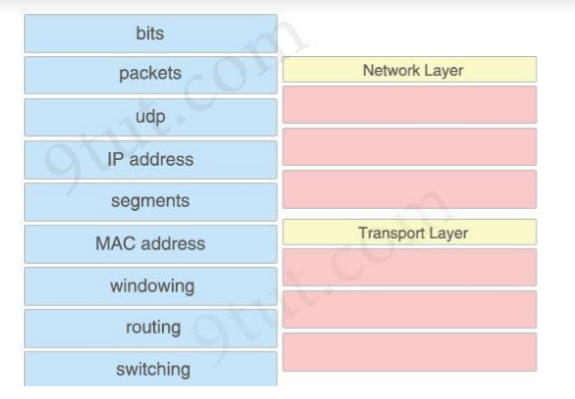
\includegraphics[width=8cm]{ta02_preg01}  
  \end{center}
  Network Layer
  \begin{itemize}
    \item packets
    \item routing
    \item Ip address
  \end{itemize}
  Transport Layer
  \begin{itemize}
    \item Segments
    \item UDP
    \item windowing
  \end{itemize}
  \item \textbf{Which command can you use to set the hostname on a switch?}
  \begin{enumerate}[label=\textbf{\Alph*.}]
    \item \underline{\texttt{switch-mdf-c1(config)\#hostname switch-mdf1}}
    \item \texttt{switch-mdf-c1\&gt;hostname switch-mdf1}
    \item \texttt{switch-mdf-c1\#hostname switch-mdf1}
    \item \texttt{switch-mdf-c1(config-if)\#hostname switch-mdf1}
  \end{enumerate}
  \item \textbf{What are the administrations forms in the Cisco devices?}
    \begin{enumerate}[label=\textbf{\Alph*.}]
      \item Console, auxiliar, ethernet
      \item Ethernet, serial, console
      \item \underline{Auxiliar, Console, Vitual Line}
      \item LAN, WAN, console
    \end{enumerate}
  \item \textbf{What option describes a LAN network? (choose two)}
    \begin{enumerate}[label=\textbf{\Alph*.}]
      \item Divides in segments called vlans
      \item \underline{Use the protocol 802.3 (ethernet)}
      \item \underline{Use the broadcast message}
      \item Don´t use broadcast message
    \end{enumerate}
\end{enumerate}

\end{document}
